\chapter{Implementation}

\section{Analysis}

\section{Approach}

\begin{figure}[h]
 \centering
 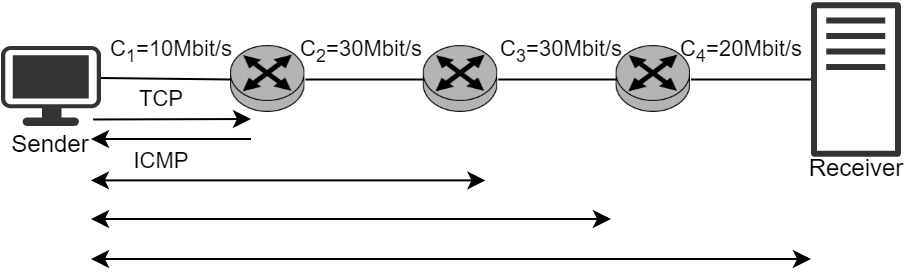
\includegraphics[width=\textwidth]{approach}
 \caption{The basic idea of the capacity estimation method}
 \label{approach}
\end{figure}



\section{Traffic Generation}

\begin{lstlisting}[language=C]
int i = 0;
while (1)
{
    //Send the packet
    if (sendto (s, datagram, iph->tot_len, 0, (struct sockaddr *) &sin, sizeof(sin)) < 0)
    {
        perror("sendto failed");
    }
    //Data sent successfully
    else
    {
        printf("%d \t", i+1);
        printf ("Packet Sent. Length: %d \n", iph->tot_len);
    }
    
    // ttl should be incremented after every n packets
    i++;
    if(i == packets) // number of packets necessary for measuring
    {
        printf("hop #%d done\n\n", iph->ttl);
        iph->ttl++;
        i = 0;
    }
    
    if(iph->ttl == routers+2) // total number of routers + 2
    {
        break;
    }
}
\end{lstlisting}


\section{Capturing the Traffic and Estimating Capacities}

